\documentclass[11pt]{article}
%\usepackage{siunitx}
\usepackage{lorig}
\usepackage{dsfont}

\let\oldphi\phi
\renewcommand{\phi}{\varphi}

\newenvironment{soln}{\begin{proof}[\textsc{Solution}]}{\renewcommand{\qedsymbol}{$\blacklozenge$}\end{proof}}

\title{Poisson Point Processes}
\author{Matt Lukac\thanks{\textbf{email:} mlukac@uoregon.edu}}
\date{\today}
\begin{document}
\maketitle
Recall a realization of the basic noise for Gaussian processes looked like that in Figure \ref{fig:gaussnoise}. Now, arrows are either muted or (rarely) point up. See Figure \ref{fig:poisnoise}.
\begin{figure}
	\centering
	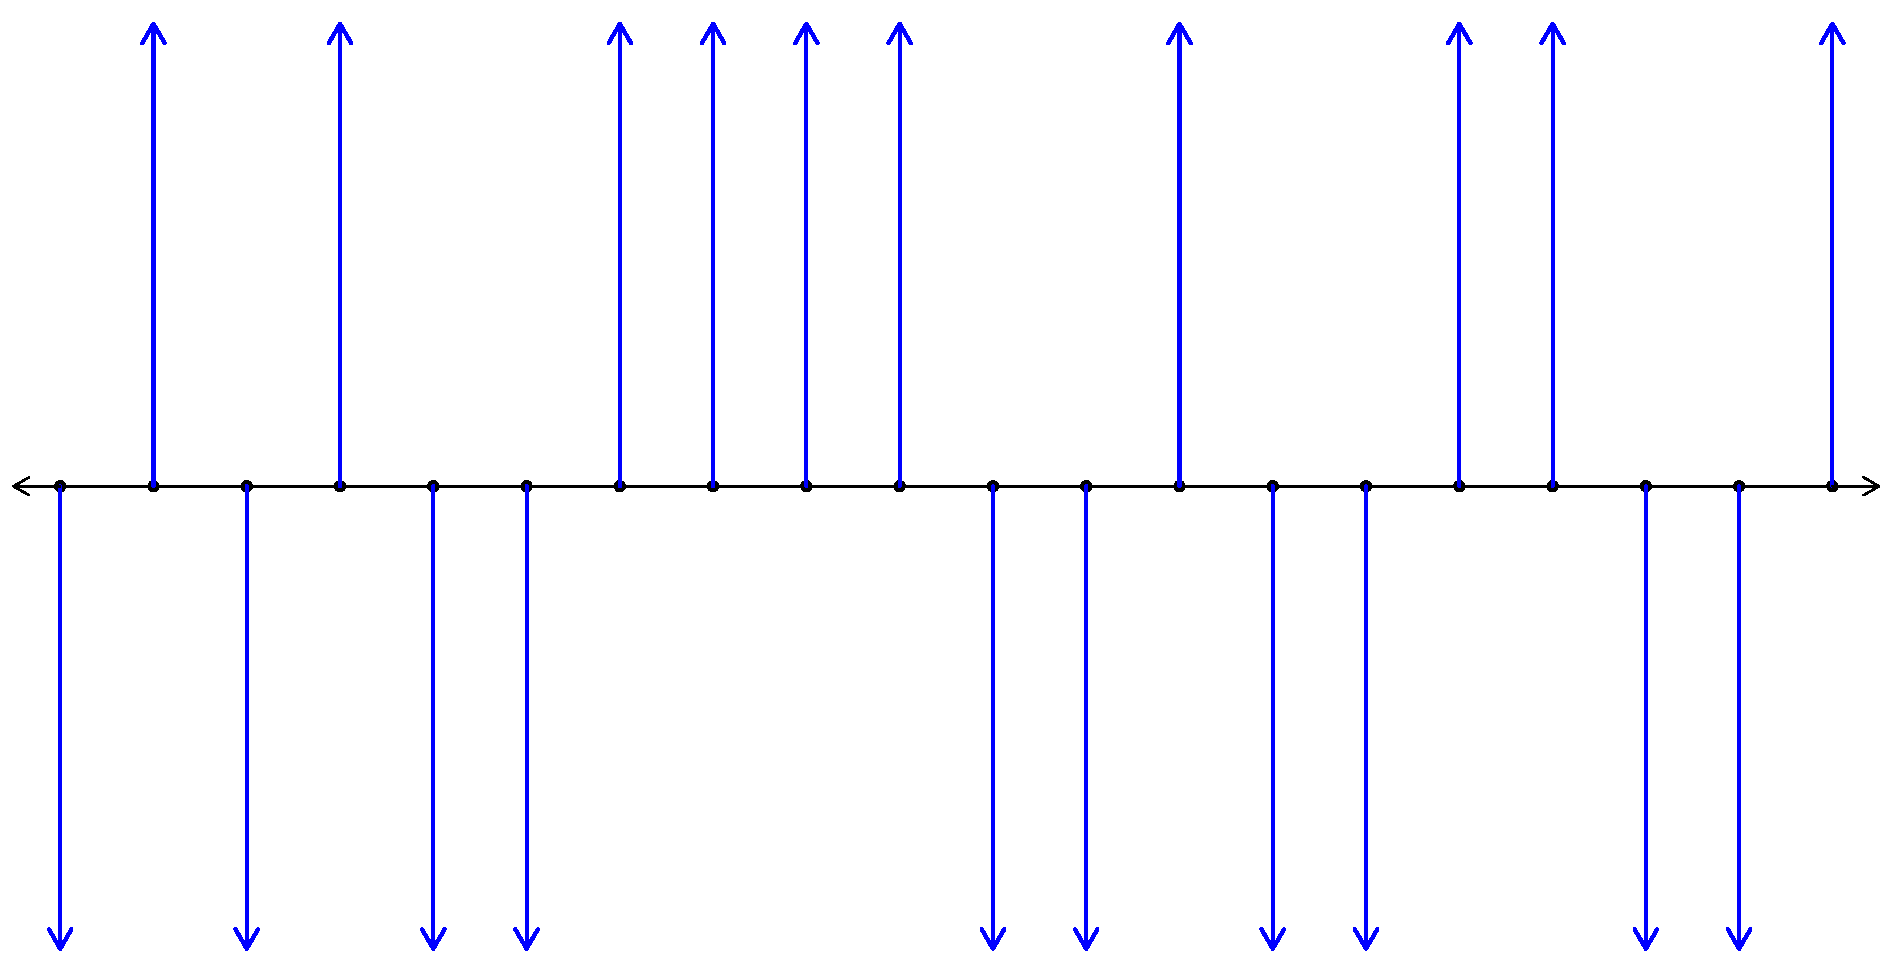
\includegraphics[width=0.9\linewidth]{gauss_noise}
	\caption{A realization of the basic noise used to construct a Gaussian process.}
	\label{fig:gaussnoise}
\end{figure}
\begin{figure}
	\centering
	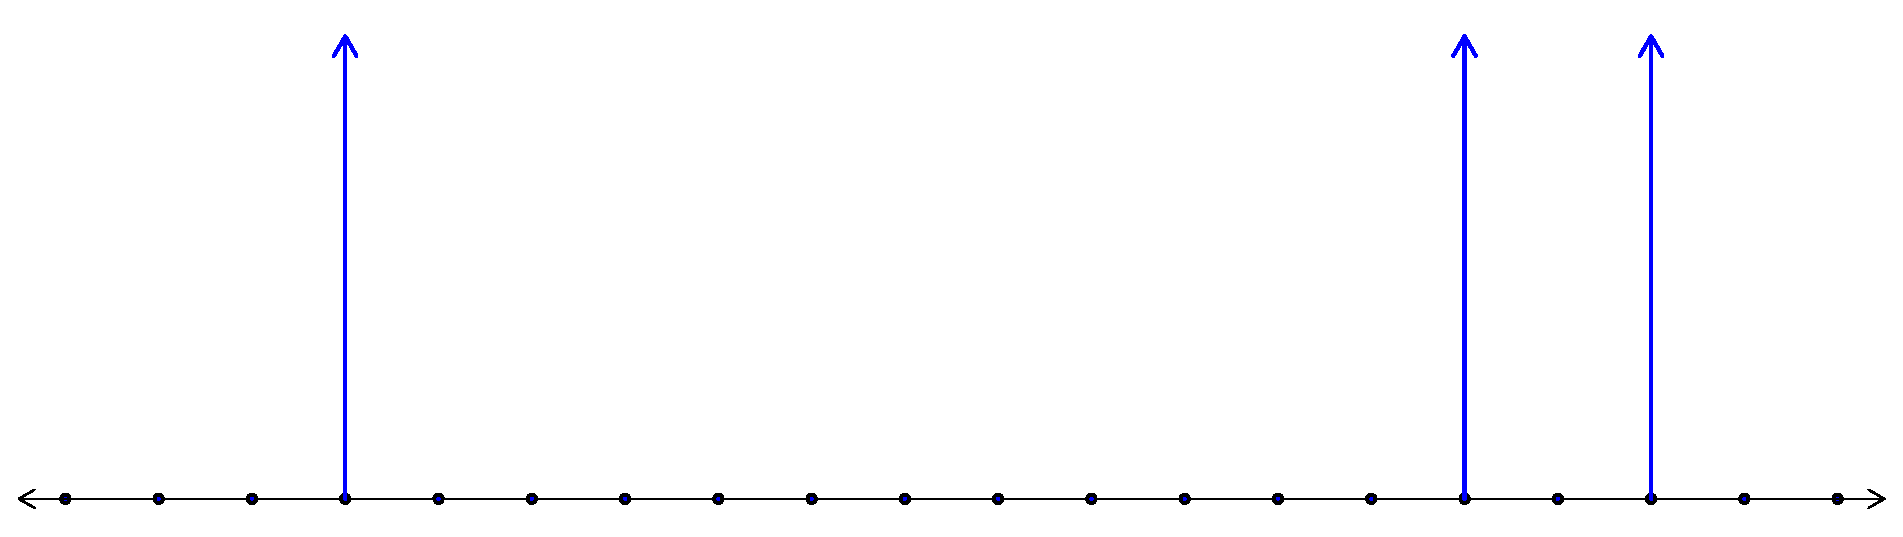
\includegraphics[width=0.9\linewidth]{pois_noise}
	\caption{A realization of the basic noise used to construct a Poisson process.}
	\label{fig:poisnoise}
\end{figure}

\section{Motivation}
Suppose in some space $X$ we lay down a large number of LED lights, each with their own battery, with density given by a $\sigma$-finite measure $\mu$. We do this in a way so that, for each region $A\subset X$, we put down about $M\mu(A)$ lights in that region, where $M$ is some large number. Independently we turn on each light with probability $M^{-1}$, and leave off otherwise.

We would like to answer the following question: how many lights in $A$ are on? To that end, let $N(A)$ denote the number of lights on in $A$ and compute
\begin{align}
	\mathbb{E}\left[ N(A) \right] = \mathbb{E} \left[ \sum_{\text{lights in }A} \mathds{1}_{\{\text{light on}\}} \right]
	= \sum_{\text{lights in }A} \mathbb{P}\left\{ \text{light is on} \right\}
		= M \mu(A) \left(\frac{1}{M}\right)
		= \mu(A).
\end{align}
Thus $\mu$ gives the expected density for the set of lights that are on in $A$. By construction, we know $N(A) \sim \operatorname{Binom}\left(M\mu(A),M^{-1}\right)$, and hence the distribution of $N(A)$ is approximately $\operatorname{Pois}(\mu(A))$. To see this, put $L = M\mu(A)$ and observe,
\begin{align}
	\mathbb{P}\left\{N(A) = n \right\} &= \binom{L}{n}\left(\frac{1}{M}\right)^n\left(1 - \frac{1}{M}\right)^{L-n}\\
	&= \frac{L(L-1)\cdots (L-n+1)}{n! M^n} \left( 1 - \frac{1}{M} \right)^{L-n}\\
	&\simeq \frac{1}{n!}\left( \frac{L}{M} \right)^n \exp\left( -\frac{L}{M} \right) + \mathcal{O}\left( \frac{1}{M} \right)\\
	&\simeq \frac{\mu(A)^n}{n!} e^{-\mu(A)}
\end{align}  
This motivates the following definition.
\begin{definition}
	Let $\mu$ be a $\sigma$-finite measure on some space $X$. A \emph{Poisson Point Process} (PPP) on $X$ with \emph{mean measure} (or, \emph{intensity}) $\mu$ is a random point measure $N$ such that:
	\begin{enumerate}[(a)]
		\item For any Borel set $A\subset X$, we have $N(A) \in \mathbb{Z}_{\geq 0}$ and $N(A) \sim \operatorname{Pois}(\mu(A))$, i.e.
		\begin{align}\label{eq:ppp}
			\mathbb{P}\left\{ N(A) = n \right\} = \frac{\mu(A)^n}{n!} e^{-\mu(A)}.
		\end{align}
		\item If $A$ and $B$ are disjoint Borel subsets of $X$, then $N(A)$ and $N(B)$ are independent random variables.
	\end{enumerate}
\end{definition}
Recall a point measure is just a measure whose mass is atomic. That is, if $\{x_i\}\subset X$ then a point measure is of the form
\begin{align}
	\mu = \sum_i a_i \delta_{x_i}
\end{align}
where $\delta_x$ is the unit point mass at $x$.
\section{PPP Properties}
It is sometimes useful to think of a PPP as a random collection of points. With this in mind, we list some important properties of $N\sim \operatorname{PPP}(\mu)$ on some space $X$:
\begin{itemize}
	\item \emph{Enumeration:} It is always possible to enumerate the points of $N$, i.e. there is a random collection of points $\{x_i\}\subset X$ such that
	\begin{align}
		N = \sum_i \delta_{x_i}.
	\end{align}
	
	\item \emph{Mean measure:} If $f\colon X \to \mathbb{R}$ then 
	\begin{align}\label{eq:mm}
		\mathbb{E}\left[ \int\! f(x) \, dN(x) \right] = \int f(x) d\mu(x).
	\end{align}
	\underline{Note:} This is a more general property of point processes, as any point process has a mean measure. To see \eqref{eq:mm} holds without needing $N$ to be a \emph{Poisson} point process, let $f$ be a simple function, i.e.
	\begin{align}
		f(x) = \sum_{i=1}^n f_i \mathds{1}_{A_i}(x), \qquad\text{where}\qquad X = \bigcup_i A_i,\quad A_i\cap A_j = \varnothing \text{ for } i\neq j.
	\end{align}
	Then we compute
	\begin{align}
		\mathbb{E}\left[ \int_X\! f(x) \, dN(x) \right] = \mathbb{E}\left[ \sum_i f_i N(A_i) \right] = \sum_i f_i \mathbb{E}\left[ N(A_i) \right] = \sum_i f_i \mu(A_i) = \int_X \! f(x) \, d\mu(x).
	\end{align}
	This can then be extended to arbitrary measurable functions through the standard limiting procedure.
	
	\item \emph{Thinning:} Independently discard each point of $N$ with probability $1-p(x)$ for a point at $x\in X$. The result is a $\operatorname{PPP}(\nu)$, where
	\begin{align}\label{eq:thin}
		\nu(A) = \int_A\! p(x) \, d\mu(x).
	\end{align}
	In other words, if $N = \sum_i \delta_{x_i}$ and $A_i = 1$ with probability $p(x_i)$ and $A_i = 0$ otherwise, then
	\begin{align}
		\widetilde{N} = \sum_i A_i \delta_{x_i} \sim \operatorname{PPP}(\nu).
	\end{align}
	
	\item \emph{Additivity:} If $N_1 \sim \operatorname{PPP}(\mu_1)$ and $N_2 \sim \operatorname{PPP}(\mu_2)$ are independent on $X$, then $N_1 + N_2 \sim \operatorname{PPP}(\mu_1 + \mu_2)$. In particular, if $\mathbb{P}\left\{ X = n \right\} = \frac{\lambda^n}{n!}e^{-\lambda}$ and $\mathbb{P}\left\{ Y = n \right\} = \frac{\nu^n}{n!}e^{-\nu}$ are independent, then
	\begin{align}
		\mathbb{P}\left\{ X + Y = n \right\} = \frac{(\lambda + \nu)^n}{n!}e^{-(\lambda + \nu)}.
	\end{align}
	
	\item \emph{Labeling:} For each point in a PPP,
	   associate an independent label from a space $Y$ 
	   according to some probability distribution $\nu$.
	   Let $N = \sum_i \delta_{x_i}$ for $\{x_i\}\subset X$ 
	   and let $G_1,G_2,\ldots \in Y$ be iid with density $\nu$. Then 
	\begin{align}\label{eq:label}
		\overline{N} := \sum_i \delta_{(x_i, G_i)} \sim \operatorname{PPP}(\mu\times\nu)
	\end{align}
	on $X\times Y$.
\end{itemize}
\section{Examples}
Henceforth, let $\lambda$ denote Lebesgue measure.
\begin{example}
	Let $N\sim \operatorname{PPP}(\lambda)$ on $\mathbb{R}_{\geq 0}$, where $\lambda$ is Lebesgue measure. As before, we think of the points of $N$ as `lights', here positioned on the positive reals.
	\begin{enumerate}[(a)]
		\item How far until the first light?
		\item Suppose each light is independently either red or green with probability $\frac{1}{2}$. How far until the first red light?
	\end{enumerate}
	\begin{soln}
		Let $N = \sum_i \delta_{x_i}$ and put $T = \min\{x_i\}$. Using \eqref{eq:ppp} we compute
		\begin{align}
			\mathbb{P}\left\{ T > t \right\} = \mathbb{P}\left\{ N([0,t]) = 0 \right\} = e^{-t}.
		\end{align}
		This solves part (a). For the colorblind readers, this also solves part (b). 
		
		Now let $\{\tilde{x}_i\}\subset \{x_i\}$ be the (random) set of red lights and define $\widetilde{N} = \sum_i \delta_{\tilde{x}_i}$, the point process for the red lights from $N$. By the thinning property \eqref{eq:thin}, $\widetilde{N} \sim \operatorname{PPP}\left(\frac{1}{2}\lambda\right)$. Similarly define $\widetilde{T} = \min\{\tilde{x}_i\}$ and observe
		\begin{align}
			\mathbb{P}\left\{ \widetilde{T} > t\right\} = \mathbb{P}\left\{ \widetilde{N}([0,t]) = 0 \right\} = e^{-t/2},
		\end{align}
		thus (b) is solved.
	\end{soln}
\end{example}
\begin{example}\label{ex:ant}
	Rain falls for 10 minutes on a large patio at a rate of $\nu = 5000$ drops per minute per square meter. Each drop splatters to a random radius $R$ that has an Exponential distribution, with mean 1cm, independently of the other drops. Assume the drops are 1mm thick and the set of locations of the raindrops is a PPP.
	\begin{enumerate}[(a)]
		\item What is the mean and variance of the total amount of water falling on a square with area $1 \text{m}^2$?
		\item A very small ant is running around the patio. See Figure \ref{fig:rainant}. What is the chance the ant gets hit?
	\end{enumerate}

\begin{soln}
	Let $N = \sum_i \delta_{(x_i,y_i)}$ where $(x_i,y_i)$ is the center of the $i$th drop. Take $N \sim \operatorname{PPP}(\nu \lambda)$ and let $M$ denote the number of drops in $[0,1]^2$, so that $M = N([0,1]^2) \sim \operatorname{Pois}(\nu)$. Then the total volume $V$ is 
	\begin{align}
		V = \sum_{i=1}^M \frac{\pi}{10^3}R_i^2
	\end{align}
	where $R_i$ is the radius of the $i$th drop. Note this is a sum of random variables where the number of terms is also a random variable. Thus we use Wald's equation \eqref{eq:wald} to obtain
	\begin{align}\label{eq:usewald}
		\mathbb{E}\left[ V \right] = \frac{\pi}{10^3}\mathbb{E}[M]\mathbb{E}[R_1^2] = \frac{\pi}{10^3}\cdot \nu \cdot \frac{2}{100^2} = \frac{2\pi}{10^7}\nu
	\end{align}
	
	The second step in \eqref{eq:usewald} was obtained from the fact that an exponentially distributed random variable $X$ with mean $\beta^{-1}$ has higher moments given by
	\begin{align}
		\mathbb{E}\left[ X^n \right] = \frac{n!}{\beta^n}.
	\end{align}
	This is proved by an iterated application of integration by parts, and the result gives rise to 
	\begin{align}
		\operatorname{var}\left[ X^n \right] = \mathbb{E}\left[ X^{2n} \right] - \mathbb{E}\left[ X^n \right]^2 = \frac{(2n)! - (n!)^2}{\beta^{2n}}.
	\end{align}
	The $n=2$ case will turn out to be useful when computing the variance of $V$.
	\newpage
	Indeed, to compute the variance we utilize the variance decomposition formula. Observe,
	\begin{align}
		\operatorname{var}[V] &= \mathbb{E}\left[ \operatorname{var}[V \mid M]\right] + \operatorname{var}\left[ \mathbb{E}[V \mid M ]\right]\\
		&= \mathbb{E}\left[ M\left(\frac{\pi}{10^3}\right)^2\operatorname{var}(R^2)\right] + \operatorname{var}\left[ M\left(\frac{\pi}{10^3}\right)\mathbb{E}[R^2]\right]\\
		&= \nu \left(\frac{\pi}{10^3}\right)^2 \left(\frac{20}{100^4}\right) + \nu\left(\frac{\pi}{10^3}\right)^2 \left(\frac{2}{100^2}\right)^2\\
		&= \left(\frac{\pi}{10^3}\right)^2\left(\frac{24}{100^4}\right)\nu.
	\end{align}
	This solves part (a).
	
	Now, part (b) can be solved by way of the labeling property. Here, we use the radius $R_i$ of the $i$th drop to label the point $(x_i,y_i)$. Recall the density of an Exponential random variable with mean $0.01$ is $100\exp(-100r)\,dr$. So we define a measure $\mu$ on $X:=\mathbb{R}^2\times [0,\infty)$ by
	\begin{align}
		\mu(A) = \int_A\! 100\nu\exp(-100r)\, dxdydr.
	\end{align} 
	We think of $X$ as the (closed) upper half plane in $\mathbb{R}^3$ where the third coordinate is a realization of $R$. By the labeling property \eqref{eq:label}, $\overline{N} := \sum_i \delta_{(x_i,y_i,R_i)} \sim \operatorname{PPP}(\mu)$ on $X$. For the ant to remain dry, any drop with radius $r$ must land outside the circle of radius $r$ centered at the ant. Viewed from the space $X$, we want to integrate over the cone with its tip at the ant, whose horizontal cross-section at height $r$ is a circle of radius $r$. From this we compute
	\begin{align}
		\mathbb{P}\left\{\text{ant is dry}\right\} = \mathbb{P}\left\{\overline{N}(A) = 0\right\}
		= \exp(-\mu(A))
		= \exp\left(-100\pi\nu\int_0^\infty\! r^2e^{-100r}\,dr\right)
		= \exp\left( -\frac{\pi\nu}{5000} \right).
	\end{align}
	Plugging in the given value for $\nu$ yields $\mathbb{P}\left\{\text{ant is dry}\right\} = \exp(-\pi) \approx 0.0432$. The ant had better grab an umbrella!
\end{soln}
\end{example}
\subsection{Wald's Equation}
The following is the statement of Wald's equation, taken from Wikipedia\footnote{The proof is also on Wikipedia.}.
\begin{theorem}[Wald's Equation]
	Let $(X_n)_{n\in\mathbb{N}}$ be a sequence of real-valued, independent and identically distributed random variables and let $N$ be a nonnegative integer-valued random variable that is independent of the sequence $(X_n)_{n\in\mathbb{N}}$. Suppose that $N$ and the $X_n$ have finite expectations. Then
	\begin{align}\label{eq:wald}
		\mathbb{E}\left[ \sum_{i=1}^N X_i \right] = \mathbb{E}\left[N \right]\mathbb{E}\left[ X_1\right].
	\end{align}
\end{theorem}
\begin{figure}
	\centering
	\label{fig:rainant}
	\caption{A realization of the ant from Example \ref{ex:ant}. Looks like he had an umbrella after all.}
	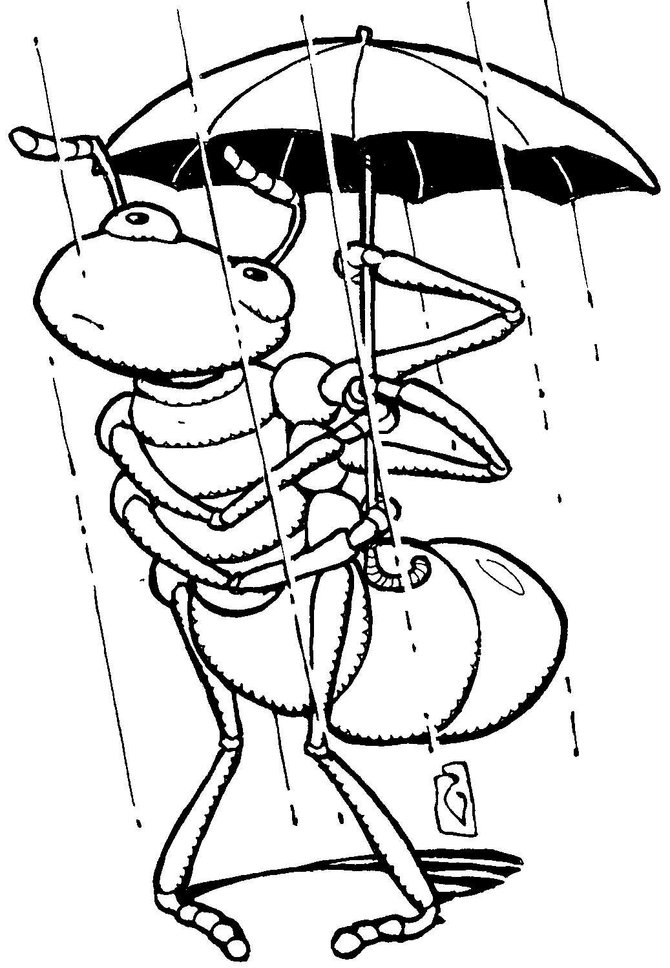
\includegraphics[width=0.7\linewidth]{rain_ant}
\end{figure}
\end{document}